\documentclass[10pt,a4paper]{article}
\usepackage[utf8]{inputenc}
\usepackage[german]{babel}
\usepackage{mathrsfs}
\usepackage{amsmath}
\usepackage{amsfonts}
\usepackage{amssymb}
\usepackage{amsthm}
\usepackage[left=2cm,right=2cm,top=2cm,bottom=2cm]{geometry}
\usepackage{graphicx}

\begin{document}

\section{Aufgabe 1}

\subsection{Teil a}

\subsubsection{(i)}

\begin{align*}
  sp(w) & = w & \textit{wenn $w \in \Sigma$}\\
  sp(aw) & = w \cdot sp(a) & \textit{wenn $w \in \Sigma$ und $a \in \Sigma^{*}$}
\end{align*}

\subsubsection{(ii)}

\begin{align*}
  |w|_{x} & = 1 & \textit{wenn $w \in \Sigma$ und $w = x$}\\
  |w|_{x} & = 0 & \textit{wenn $w \in \Sigma$ und $w \ne x$}\\
  |wa|_{x} & = |w|_{x} + |a|_{x} & \textit{wenn $w \in \Sigma$ und $a \in \Sigma^{*}$}
\end{align*}

\subsection{Teil b}

\subsubsection{(i)}

\begin{equation}
  L_{1} = \{ \lambda \}, L_{2} = \{ 0, 11, 0011 \}
\end{equation}
\begin{equation}
  L_{1} = \{ 0, 11, 0011 \}, L_{2} = \{ \lambda \}
\end{equation}

\subsubsection{(ii)}

\begin{equation}
  L_{1} = \{ \lambda \}, L_{2} = \{ 0, 011, 0011 \}
\end{equation}
\begin{equation}
  L_{1} = \{ 0 \}, L_{2} = \{ \lambda, 11, 011 \}
\end{equation}
\begin{equation}
  L_{1} = \{ 0, 011, 0011 \}, L_{2} = \{ \lambda \}
\end{equation}

\section{Aufgabe 2}

\subsection{Teil a}
\begin{equation}
  G_{\mathbb{N}} = (\Sigma'', \{ S, C \}, S, P)
\end{equation}
P enthält die Regeln
\begin{align*}
  S & \mapsto 1C | 2C | 3C | 4C | 5C | 6C | 7C | 8C | 9C\\
  S & \mapsto 1 | 2 | 3 | 4 | 5 | 6 | 7 | 8 | 9\\
  C & \mapsto 0C | 1C | 2C | 3C | 4C | 5C | 6C | 7C | 8C | 9C\\
  C & \mapsto 0 | 1 | 2 | 3 | 4 | 5 | 6 | 7 | 8 | 9
\end{align*}

\subsection{Teil b}

\begin{equation}
  G_{\mathbb{Z}} = (\Sigma', \{ S, N, Z \}, S, P)
\end{equation}
P enthält die Regeln
\begin{align*}
  S & \mapsto -N | N\\
  N & \mapsto 0 | 1Z | 2Z | 3Z | 4Z | 5Z | 6Z | 7Z | 8Z | 9Z\\
  Z & \mapsto 0 | 1 | 2 | 3 | 4 | 5 | 6 | 7 | 8 | 9\\
  Z & \mapsto 0Z | 1Z | 2Z | 3Z | 4Z | 5Z | 6Z | 7Z | 8Z | 9Z
\end{align*}

\subsection{Teil c}

Siehe Teil e.
Da diese Typ 3 ist, ist sie auch Typ 2.

\subsection{Teil d}

\begin{equation}
  w_{1} = S \vdash N \vdash 1L \vdash 1/R \vdash 1/4Q \vdash 1/43Q \vdash 1/432
\end{equation}
\begin{equation}
  w_{2} = S \vdash N \vdash 4Z \vdash 43Z \vdash 432Z \vdash 4323Z \vdash 43231L \vdash 43231/R \vdash 43231/1
\end{equation}
\begin{align*}
  w_{3} = S & \vdash -N \vdash -5Z \vdash -54Z \vdash -542Z \vdash -5420L \vdash -5420/R\\
  & \vdash -5420/2Q \vdash -5420/22Q \vdash -5420/221Q \vdash -5420/2213
\end{align*}

\subsection{Teil e}

\begin{equation}
  G'_{\mathbb{Q}} = (\Sigma, \{ S, N, Z, L, R, Q \}, S, P)
\end{equation}
P enthält die Regeln
\begin{align*}
  S & \mapsto -N | N\\
  N & \mapsto 0L | 1L | 2L | 3L | 4L | 5L | 6L | 7L | 8L | 9L | 1Z | 2Z | 3Z | 4Z | 5Z | 6Z | 7Z | 8Z | 9Z\\
  Z & \mapsto 0L | 1L | 2L | 3L | 4L | 5L | 6L | 7L | 8L | 9L | 0Z | 1Z | 2Z | 3Z | 4Z | 5Z | 6Z | 7Z | 8Z | 9Z\\
  L & \mapsto /R\\
  R & \mapsto 1 | 2 | 3 | 4 | 5 | 6 | 7 | 8 | 9 | 1Q | 2Q | 3Q | 4Q | 5Q | 6Q | 7Q | 8Q | 9Q\\
  Q & \mapsto 0 | 1 | 2 | 3 | 4 | 5 | 6 | 7 | 8 | 9 | 0Q | 1Q | 2Q | 3Q | 4Q | 5Q | 6Q | 7Q | 8Q | 9Q\\
\end{align*}

\section{Aufgabe 3}

\subsection{Teil a}

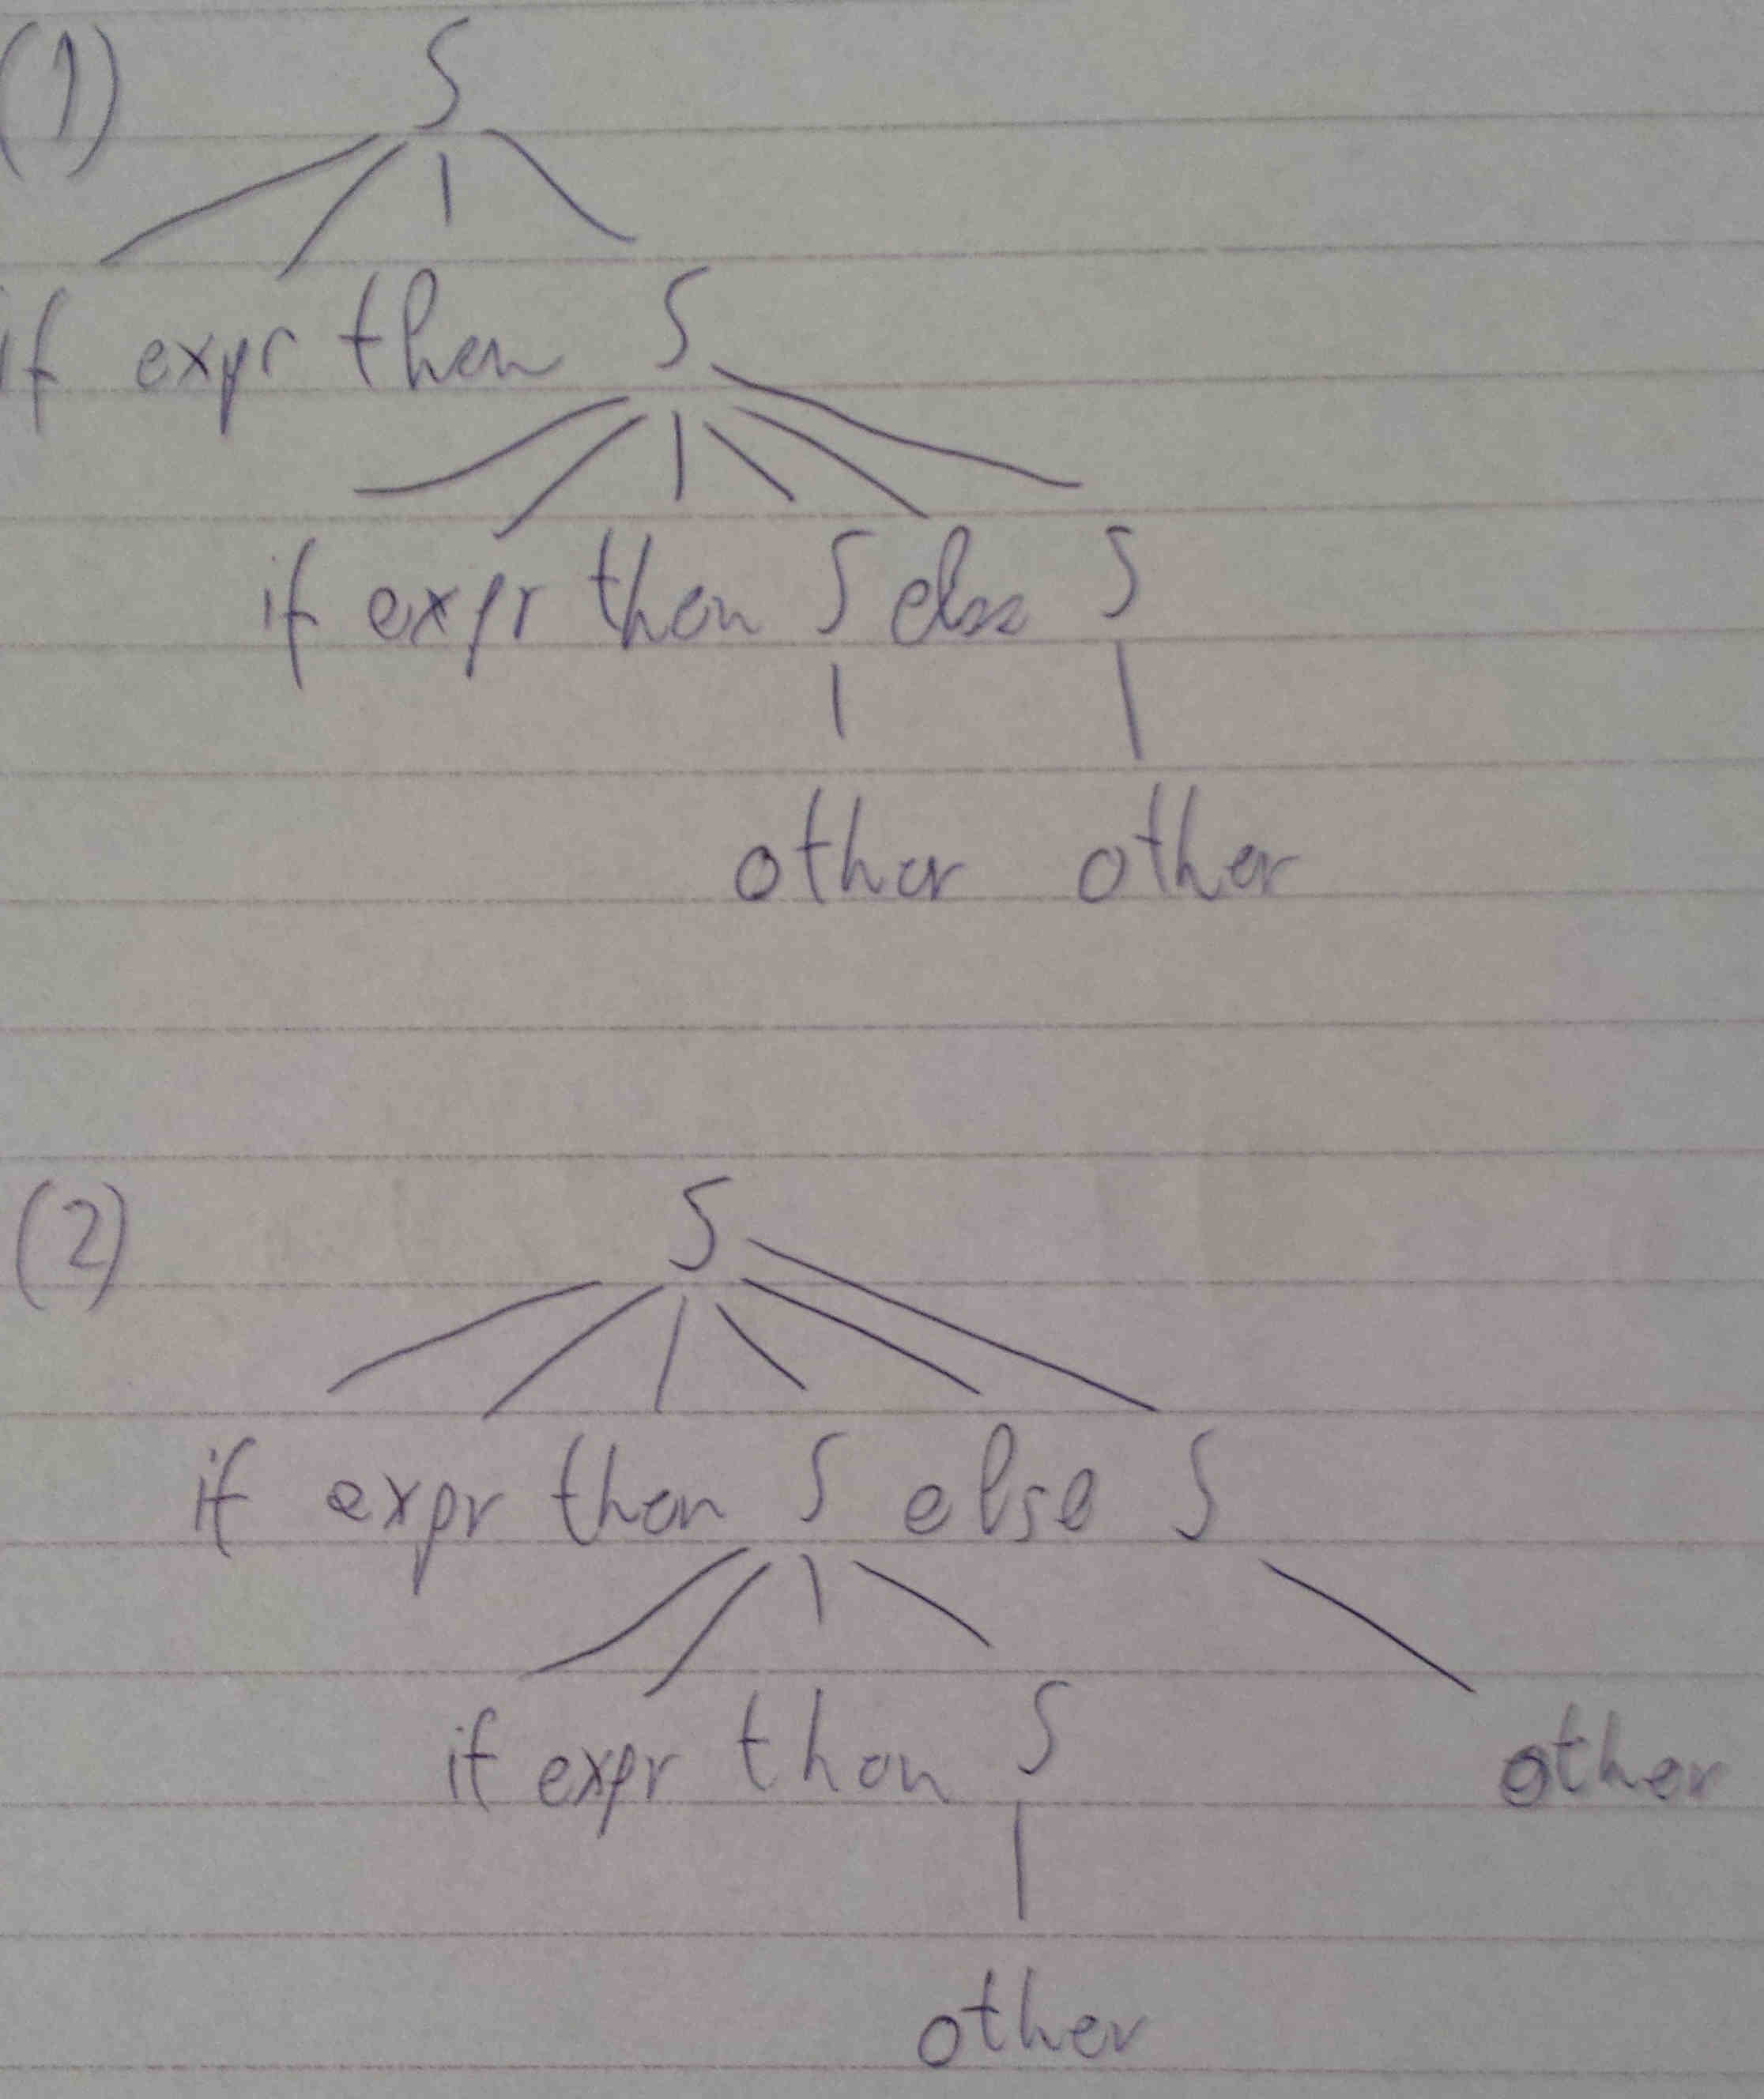
\includegraphics[width=250pt]{3_a.jpg}

\subsection{Teil b}

if expr then if expr then other else if expr then other else other

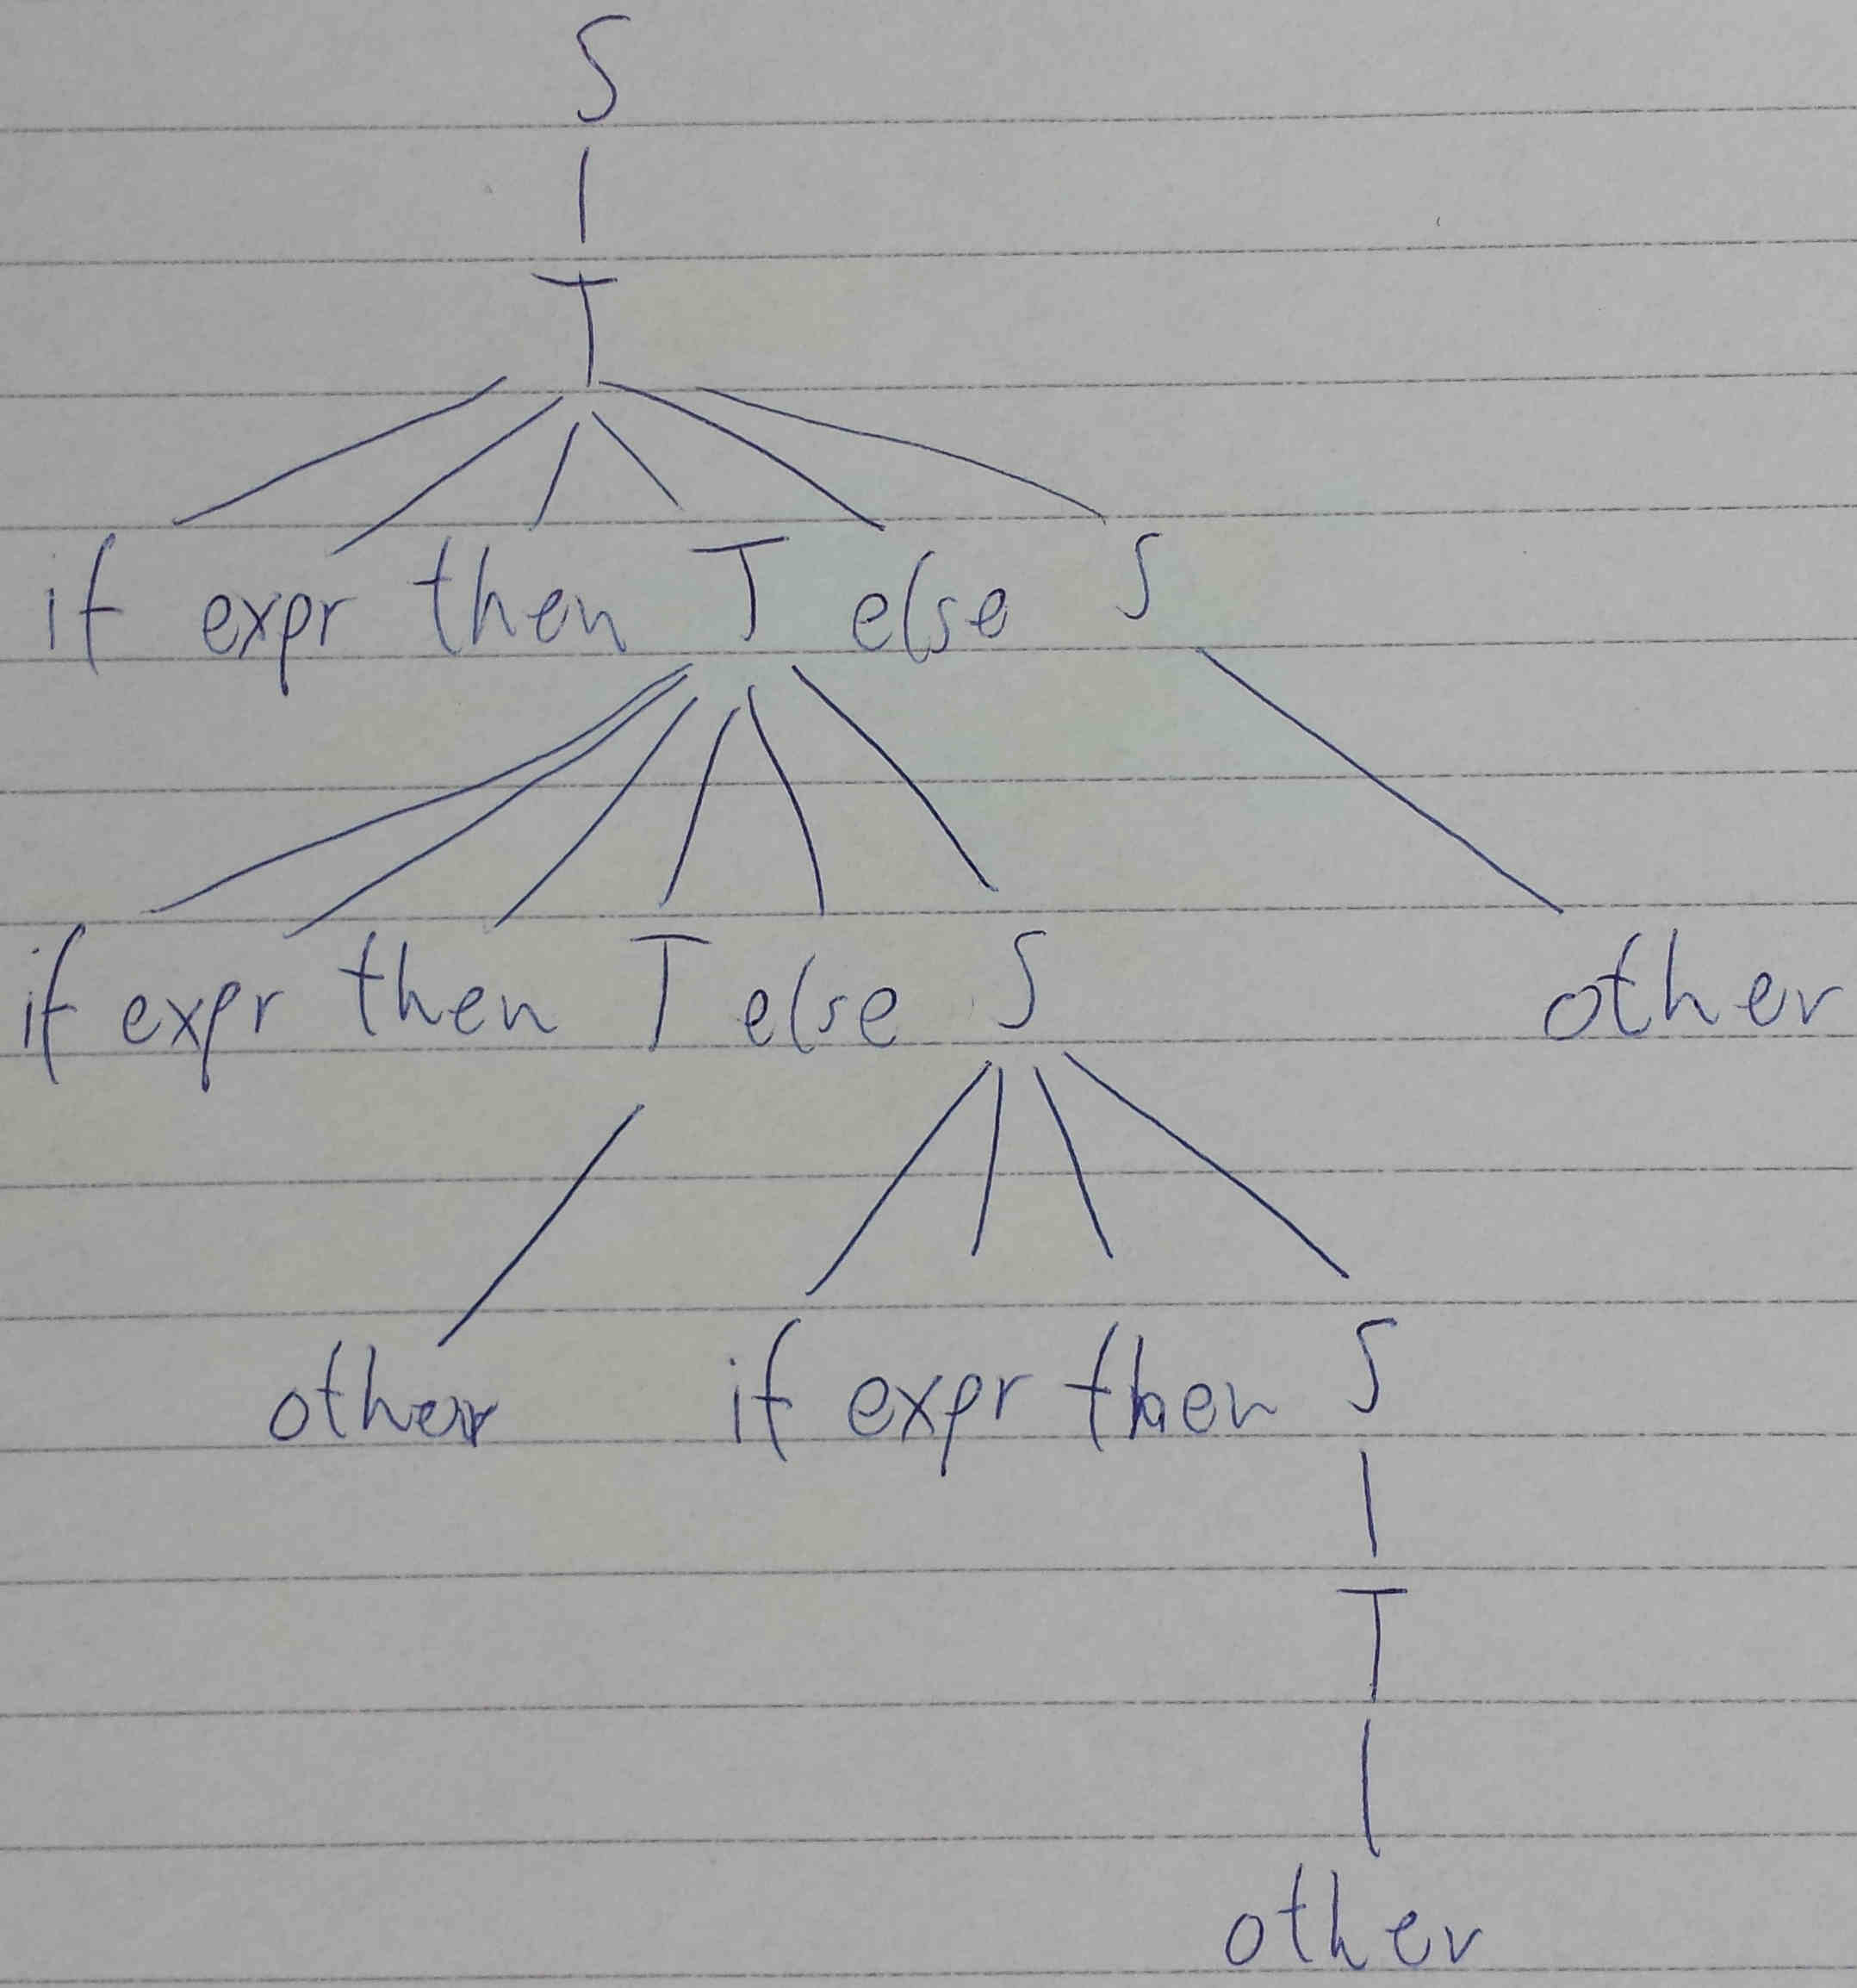
\includegraphics[width=250pt]{3_b_1.jpg}
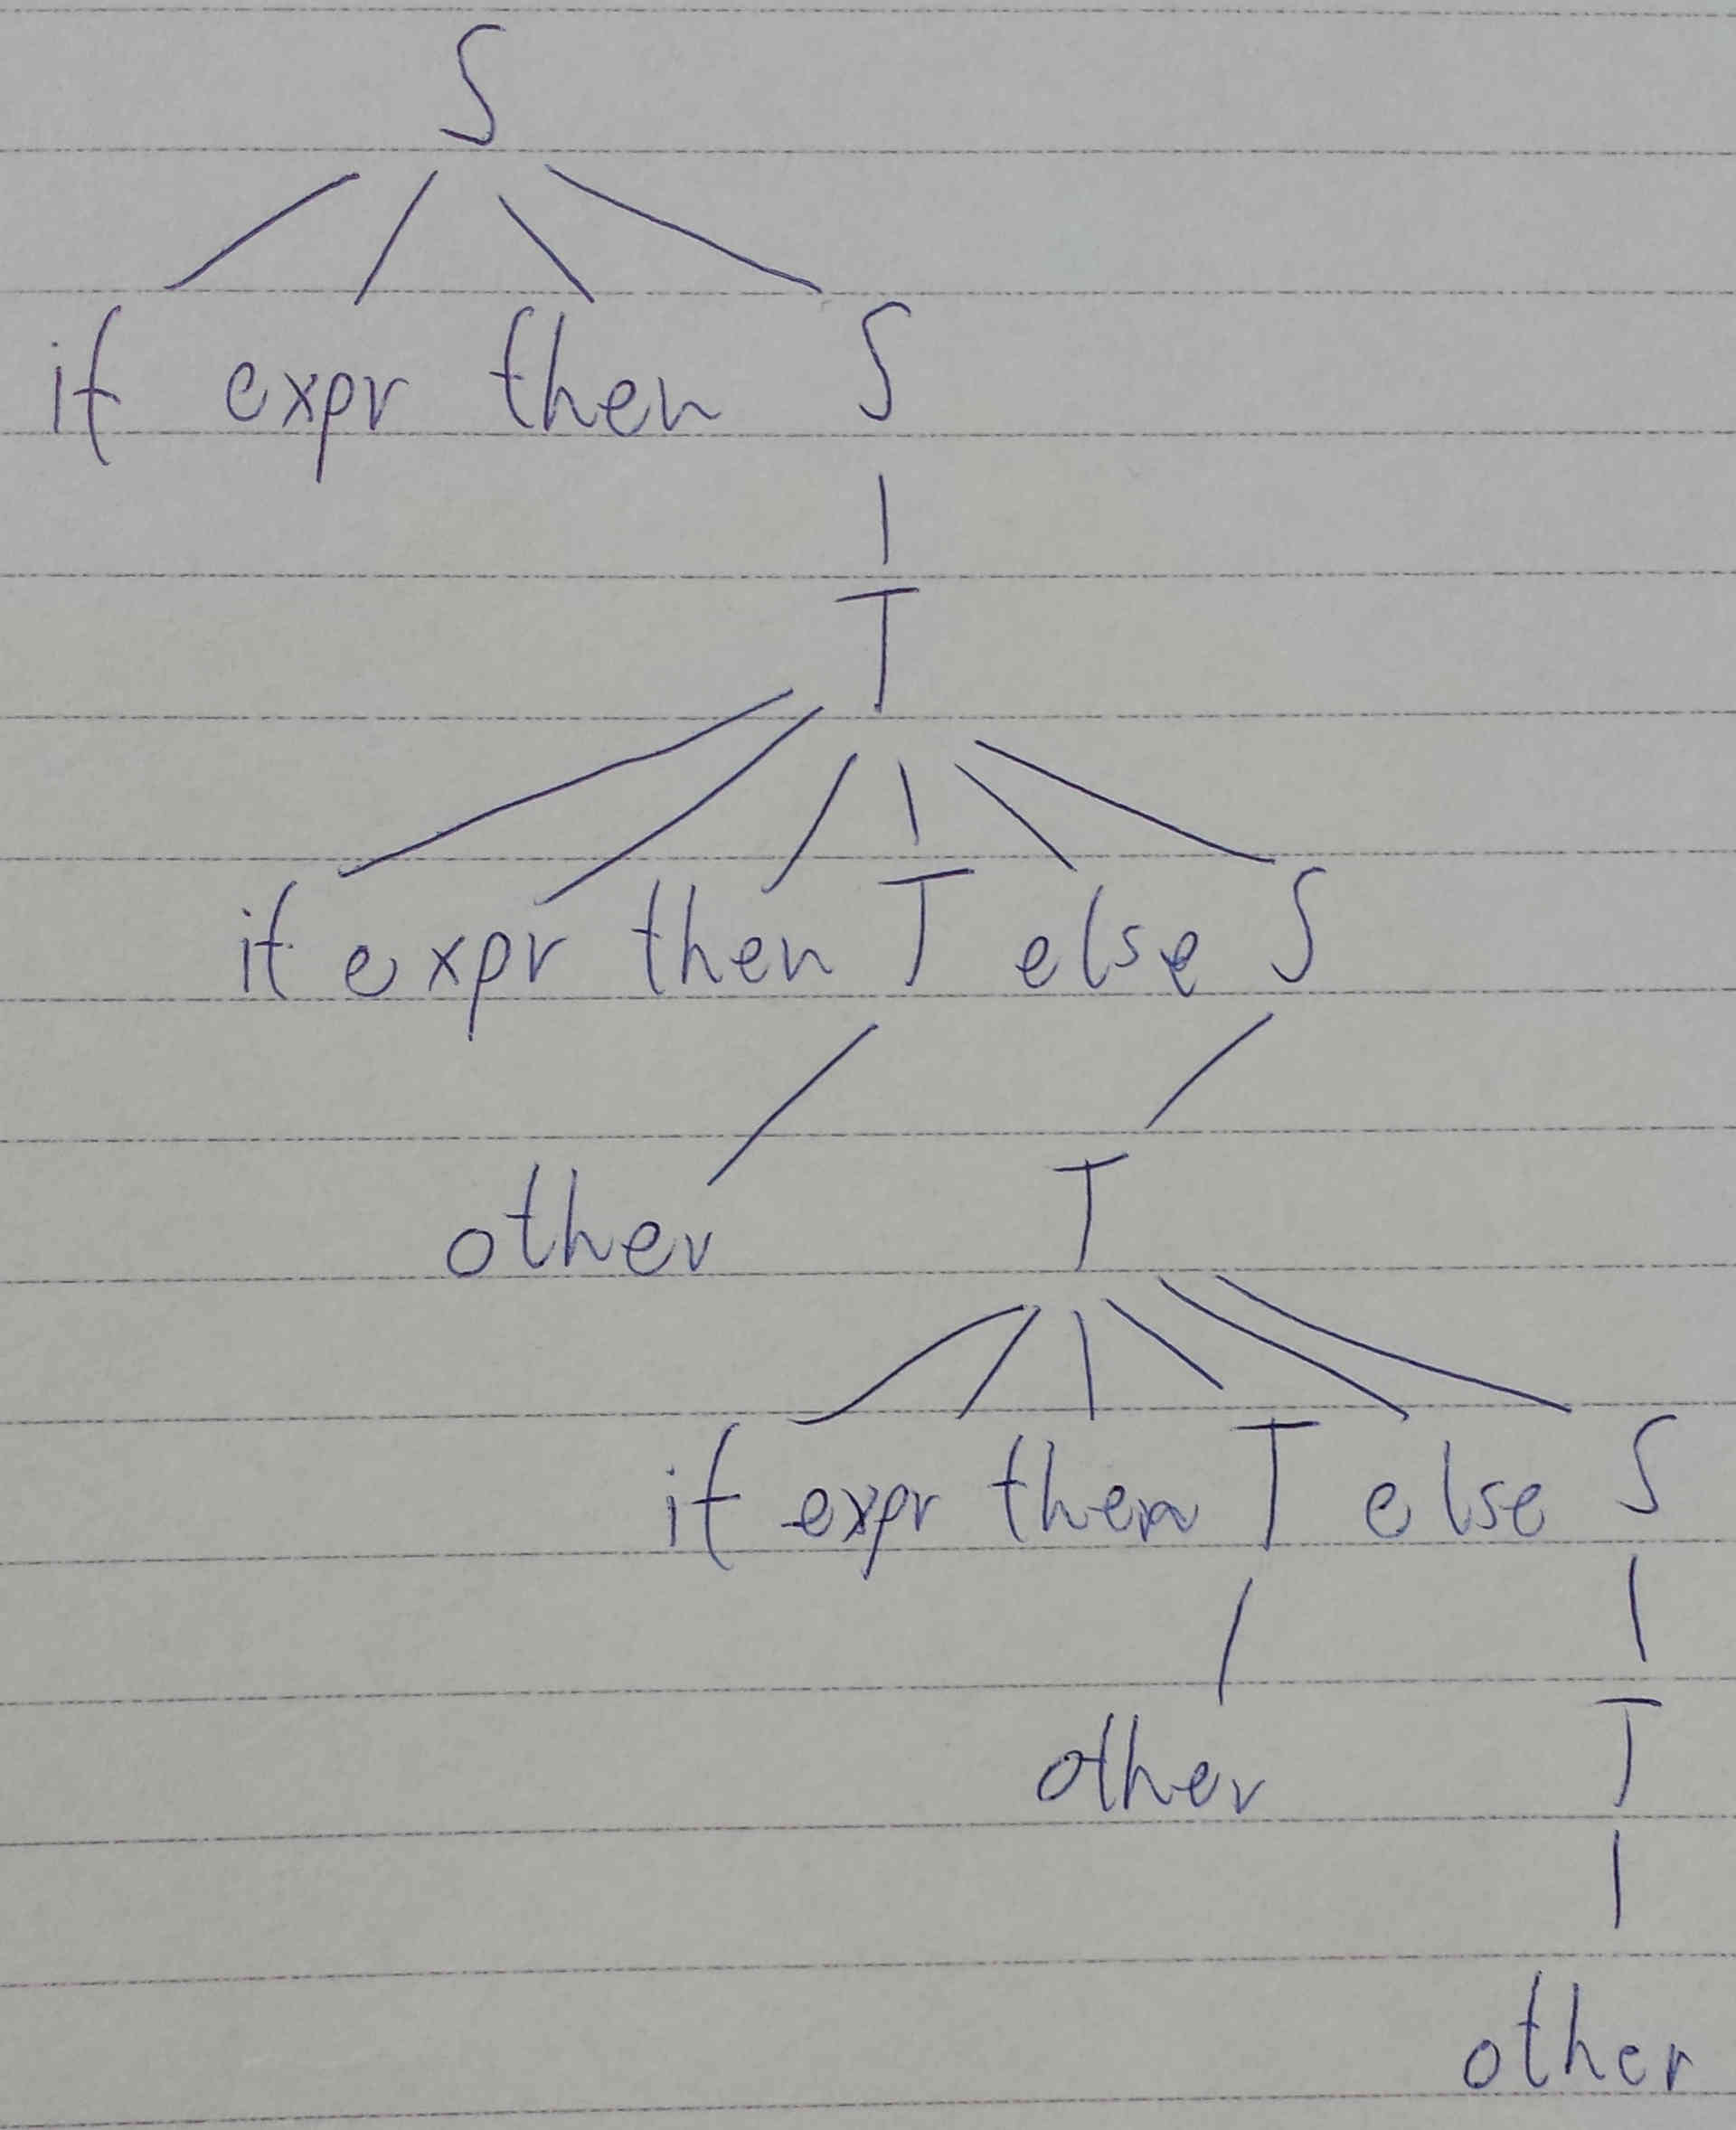
\includegraphics[width=250pt]{3_b_2.jpg}

\end{document}